
\chapter{Context}

\label{Context} 

% LC 43 References

%This chapter explains the current state of your topic, in practice and theory. This is the state of the world which you intend to improve, and the state of knowledge on top of which you build your advances and from which you learn knowledge to apply and constraints on your work. So, you will report and analyse what is known about a certain topic, as reported in reference literature and published scientific literature; if you are developing a product, you will need to report about comparable or competing products over which you intend to improve or from which you will obtain ideas; you may need to describe legal or societal situation within which your work takes place; etc.  
  
%It is important to demonstrate scholarship, i.e. the ability to read about a subject area in a range of sources, assimilate the material and then discuss it intelligently.  
  
%You should demonstrate that you understand what you have read by providing some analysis or commentary in view of the goals of your project: it is not enough simply to provide summaries of what you have read. References should be cited following the Harvard Referencing Style. You must also explain, both in this chapter and, as appropriate, in others, how the results of the studies to which you make reference inform your project work. To gain a passing grade, your report MUST demonstrate adequate engagement with academic literature and any other sources necessary for the work to be well informed.  

% The story we want to tell
% End to end learning - what does it mean
% Describe pipelined methods, contrast and compare to end to end methods

% Datasets and the importance of large public datasets for deep learning
% Synthetic datasets - how these become important as data can be difficult and costly to acquire

%% Prior methods used in image classification, using manual feature extraction

% Data dirth, not dirt, and network performance
% Augmentation
% Mechanical Turk to the rescue
% Large public datasets
% Public self driving datasets, large, but aimged at pipeline models

% What is end to end learning?

%%%%%%%%%%%%%%%%%%%%
% RELATED WORK
%%%%%%%%%%%%%%%%%%%%

\section{Related Work}

Adverse weather affecting sensor data including cameras used by AVs was surveyed by \cite{ZangAdverseWetherAVSurvey8666747}.  
\cite{ClearingSkiesDeepNNRainRemoval7893758}
\cite{Cord2014DetectingUR}, determining that video-camera based ADASs (Advanced driver assistance systems) are becoming ever present in the automotive sector. The trade off being good performance in good weather \textit{versus} bad performance in bad weather, particularly in the rain. The suggested approach is to detect unfocused raindrops on the vehicle's windscreen, using in-vehicle camera images. Then analyse raindrop photo metric properties and rely on image processing to highlight the rain drops. This technique is claimed to improve ADAS behaviour in the rain.  
  
\cite{yoneda2019automated} acknowledge the possibility of object recognition performance degradation due to image quality degradation, and suggest careful positioning of camera inside the vehicle within windscreen wiper range. It is also acknowledged that this may not be a possibility if the camera is place on the side or outside of the vehicle to capture images in every direction, the raindrops then being inevitable, concluding that when camera installation is performed, raindrops and a mechanism for removal are required. Research on rain-drop recognition in the captured image is reported.

\cite{kurihata2005rainy} suggest a method for weather recognition with images being captured from in-vehicle camera able to use a subspace method to asses rain by detecting rain drops on the windshield.
\textit{Eigendrops} represent the a form of PCA (principal component analysis), extracting from components from raindrop images in the learning stage. Then template matching is used to detect rain drops. The authors claim the method showed good results with video sequences containing raindrops and promising detection results for rainfall judgement 
  
\cite{webster2015improved} state image containing raindrops are prone to distortion as rain has a significant negative performance impact in a wide range of sensing applications based on visual sensing and used in all weather conditions including surveillance and vehicle autonomy. The problem is framed as "robust raindrop detection" as a means of identifying the potential for performance degradation in affected image regions. Raindrop detection is colour video is performed using "extended feature descriptor comprising localised shape".
  
\cite{garg2007vision} state rain produces complex visual effects such as sharp intensity changes, that can severely compromise performance of outdoor vision systems, providing a comprehensive analysis of visual effects of rain and various related factors such as camera parameters, rain properties, brightness.
  
Related work was therefore found studying the  effect of rain on sensors specifically, applicable to multi-sensor fusion models (see next section). All literature surveyed frame the problem in terms being solved with a manual feature extraction solution, in other works, no mention is made of CNNs. No literature related to the effect of rain on CNNs was found.

%%%%%%%%%%%%%%%%%%%%%%%%%%%%%%%%%%%%%%%%%%%%%%%%%%%%%%%%
% Self driving systems
%%%%%%%%%%%%%%%%%%%%%%%%%%%%%%%%%%%%%%%%%%%%%%%%%%%%%%%%
\section{Self-driving systems}
The "Dave" system, \cite{lecun2004dave}, was a proof-of-concept, model scale vehicle that used end-to-end learning for obstacle avoidance, based solely on two onboard cameras equipped with analogue video transmitter and a remote computer to process the image data and send back steering control signals via radio. On the remote computer, YUV images (\cite{maller2020}) from left and right cameras were presented to a network trained to output steering angles. Hours of binocular video images, labelled with a steering angle provided by a human driver, who avoided any obstacles found to be in path, were used to train the network.

Figure \ref{fig:bojarski-net}
% bojarski
shows a diagram representing a CNN predicting a steering angle from a single  front-facing camera. The NVIDIA PilotNet (\cite{bojarski2016end}) was able to learn to drive on local roads with or without road markings, and also operate in areas with unclear markings such as parking lots. Like Dave, this is another example of end-to-end learning, with no intermediate criteria such as lane detection. The authors state such criteria is devised solely to simplify human understanding, but does not necessary translate into system performance. Features are instead extracted automatically by convolutional layers on the network, the fully connected layers then performing the classification or regression task as needed.

\begin{figure}[ht]
 \centering 
 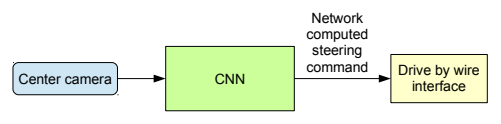
\includegraphics[scale=1]{Figures/bojarski-nvidia.png}
 \caption{Diagram of a trained network with a single centre camera input and a steering command output}
 \label{fig:bojarski-net}
\end{figure}

One weakness of convolutional neural networks is the perceived lack of robustness. Figure \ref{fig:one-pixel-attack} shows examples of a \textit{one-pixel attack} (\cite{Su_2019}). The attackers did have a deep knowledge of the network architecture being exploited, still in this classification task setting it is an undesirable outcome.


\begin{figure}[ht]
 \centering 
 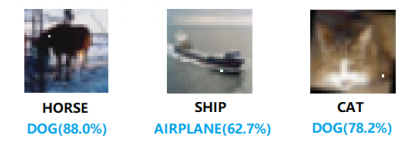
\includegraphics[scale=1]{Figures/one-pixel-attack.png}
 \caption{One-pixel  attacks  created  with the algorithm proposed by \cite{Su_2019} that  successfully  fooled  three  types  of deep neural networks trained  on  CIFAR-10 (\cite{CIFAR_10}) dataset. The modified pixel is white, the original  class  labels  are   black while  the  target  class  labels  and  the corresponding confidence are blue}
 \label{fig:one-pixel-attack}
\end{figure}

Another scheme used for self-driving cars is the multisensor (\cite{Grigorescu_2020} and \cite{Yurtsever_2020}) approach shown in Figure \ref{fig:grigorescu-pipeline}, where a number of number of input configurations can potentially be used, with of without deep learning, that is with the help of a multilayer neural network with a least one hidden layer. The approach may use classical "rules based" programming to determine steering and motion.

\begin{figure}[ht]
 \centering 
 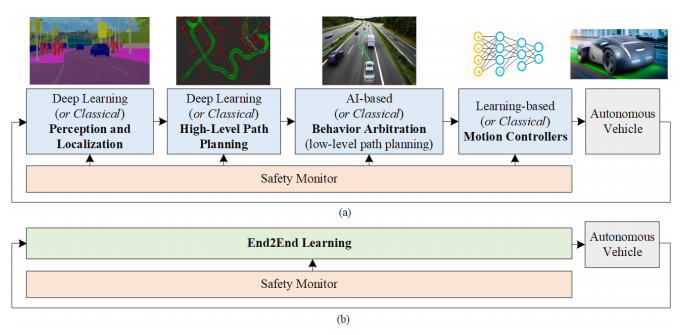
\includegraphics[scale=0.85]{Figures/grigorescu-pipeline.png}
 \caption{Diagrams showing the multisensor pipeline approach (a) and the end to end approach (b) as described by \cite{Grigorescu_2020}}
 \label{fig:grigorescu-pipeline}
\end{figure}


The introduction of any AI-controlled hardware into public spaces also raises a number of societal issues like safety, liability, privacy, cybersecurity, and industry (\cite{Taeihagh_2018}).
Other issues include the impact on demand for a human workforce, wages and employment (\cite{acemoglu2018artificial}).


%%%%%%%%%%%%%%%%%%%%%%%%%%%%%%%%%%%
% Netowrk Training
%%%%%%%%%%%%%%%%%%%%%%%%%%%%%%%%%%%

\section{Network Training}

%%%%%%%%%%%%%%%%%%%%%%%%%%%%%%%%%%%%%%%%%%%%%%%%%%%%%%%%
% Properties of  multilayer feedforward neural networks
%%%%%%%%%%%%%%%%%%%%%%%%%%%%%%%%%%%%%%%%%%%%%%%%%%%%%%%%

The properties of multilayer feedforward neural networks as universal function approximators has been studied extensively, especially in the 1980's. \cite{hornik1989multilayer} rigorously established that standard multilayer feedforward networks with as few as one hidden layer can approximate specific functions provided sufficiently many hidden units are available, though the issue of how many are required is not addressed. \cite{cybenko1989approximation} demonstrated analytically that a feedforward neural network with one hidden layer and any continuous sigmoidal nonlinearity can approximate any function with arbitrary precision provided that
no constraints are placed on the number of nodes or the size of the weights. As such, failures in applications can be attributed to inadequate learning, inadequate numbers of hidden units, or the presence of a  stochastic rather than a deterministic relation between input and target.
Training will therefore fail due to inadequate learning or hidden unit number choices, or the existence of a stochastic, non-deterministic, relation between input and target. 

The goal is to find optimal parameters (weights and biases) and biases for a arbitrary size multilayer, or deep network, because as the depth or width increases, so do the number of parameters.  

Changes in network parameter distribution during training lead to a changes in network activation distributions, this is known as Internal Covariate Shift (\cite{ioffe2015batch, 7005077}). \cite{lecun1998gradient}; \cite{wiesler2011convergence}, suggest a long known method to address the issue by linearly transforming input values to have zero mean and unit variance. To achieve this, the pixel values (maximum value 255) are divided by 255 and have 0.5 subtracted, such that transformed values will have "whitened" zero mean and unit variance. This is done repeatedly throughout the training. By fixing the distribution of the inputs, training speed is expected to improve.
Networks trained which such inputs must also be presented with whitened inputs at inference (prediction) time.

The inputs are affected by weights and biases in all the previous layers, changes in the inputs during training will lead to saturation, also known as vanishing gradients (weights and biases becoming very large or small), the effect increasing with network depth (deep networks) . Several schemes have been used to address this saturated regime: adequate parameter initialization (\cite{glorot2010understanding}, \cite{saxe2013exact}), small learning rates
and Rectified Linear Units (\cite{nair2010rectified}).

The large search space for optimal network parameters can be addressed by a number of optimizers for example error backpropagation (\cite{rumelhart1986learning}) with Stochastic Gradient Descent that can lead to better results in large datasets where there is repetition. \cite{lecun2012efficient} suggests that examples (inputs) should be shuffled to attain maximum information content but points out this will not apply to data with outliers.

Since more data is better for network training, data augmentation can be used to increase the amount of data available to train the model (\cite{perez2017effectiveness}). This is achieved by drawing additional data from the training data itself. It can help to make the network generalise and avoid overfitting, that is, doing a good job in predicting examples that have been seen but not doing so well with unseen examples.
"Hyperparameter", a non-trainable parameter, choices can also impact accuracy. Kernel size, stride padding, activation and loss functions, and optimizers are hyperparameters than can be adjusted for best network performance.

A typical multi-class classifier CNN will have a softmax activation function in the final layer and a cross-entropy loss function. a typical regression model will have a linear activation function in the final layer and a mean squared error loss function.
To transform a deep classification model into a deep regression model, the number of class outputs is replaced by the number of required continuous outputs, the softmax activation is replaced by a linear activation and the cross-entropy loss is replace by mean squared error loss.

Class imbalance (\cite{batista2004study}) has an effect on model's accuracy. A heavily outnumbered class may be difficult to learn. Rare events lead to the creation of imbalanced learning scenarios (\cite{krawczyk2016learning}). In the case of self-driving car data, the expectation is that most of steering angle labels will be close to zero (car driving straight). So some form of undersampling of majority classes (if viewing steering angle ranges, for instance, as would be achieved by binning) may help to address the issue.
%%%%%%%%%%%%%%%%%%%%
% DAVE
%%%%%%%%%%%%%%%%%%%%
%Dave (\cite{lecun2004dave})
%Autonomous off-road vehicle control using end-to-end learning



% on calculating light intensity of RGB value

% https://computergraphics.stackexchange.com/questions/5085/light-intensity-of-an-rgb-value

% on "smoothing" with matlab code provided:
% https://www.researchgate.net/profile/Manu_Bn2/publication/295235499_Rain_Removal_From_Still_Images_Using_L0_Gradient_Minimization_Technique/links/56c847aa08ae96cdd06acb6f.pdf

% Maybe a bit of history on SVM, HOG, SURF, etc. Perhaps best in introduction, like how this was a step, where manual feature extraction was used, then came end to end applied to computer vision problems.

% Intro explain term "end to end" - move to intro

% Context - successes in deep convolutional neural networks applied to computer vision problems

% 2. Imagenet - large public dataset \cite{deng2009imagenet}

%% MODELS

% 3. Alexnet - 
% 4. VGG - \cite{simonyan2015deep}
% 5. RESNET \cite{he2015deep}
% 6. Inception \cite{szegedy2014going}

% Then NVIDIA uses a deep convolutional neural networks architecture for end to end driving, i.e. image (raw pixels) in, vehicle control out.

% 1. NVIDIA end to end \cite{bojarski2016end}, DAVE2

% 7. \cite{Su_2019} 
% 8. \cite{zhang2017understanding}

%% However, these networks do have weaknesses, as demonstrated by \cite{Su_2019} in the form of one pixel attacks.
% \cite{zhang2017understanding} % demonstrated that simple depth two neural networks already have perfect finite sample expressivity as soon as the number of parameters exceeds the number of data points as it usually does in practice
%% Such examples question the robustness of deep convolutional neural networks. Especially in the context of one pixel attacks, when small addition of random noise causes the model to completely misinterpret the results, raising questions about generalisation, overfitting and robustness of the deep neural network architectures described.

%% DATASETS

%% 9. Audi dataset https://www.a2d2.audi/a2d2/en/download.html
% \cite{geyer2020a2d2},
%% 10. Ford Multi-AV Seasonal Dataset
% \cite{agarwal2020ford}
%% 11. Udacity
%Maybe a bit on how synthetic datasets are used in other domains e.g. https://arxiv.org/pdf/1910.02550.pdf "ClearGrasp:
%3D Shape Estimation of Transparent Objects for Manipulation" use of Blender. See section "Learning from synthetic data"

%% Identifying rainy data segments - Amazon Sagemaker 
% 19. \cite{joshi2020amazon}
% Mechanical Turk
% 20. \cite{crowston2012amazon}

%% SYNTHETIC DATASETS
% Cleargrasp
% 12. \cite{sajjan2019cleargrasp}

%% TOOLS -- maybe move tools to METHODS section
%% ROS
% \cite{quigley2009ros}

%% TENSORFLOW
% 13. \cite{abadi2016tensorflow}
%% KERAS
% 14. \cite{chollet2015keras}
%% PYTORCH
% 15. \cite{NEURIPS2019_9015}

% 3D environments
% 3D gaming engines
%% UNREAL - used by INTEL/AUDI/FORD TBC
% 16. \cite{unrealengine}
% user by AIRSIM
% 17. \cite{shah2017airsim}

%% UNITY - used by Udacity
% 18. \cite{haas2014history}

% Blender used to create synthetic datasets
% 21. \cite{rajpura2017object}

%% Public datasets
%Kaggle (\cite{kaggle_2020} contains over 50,000 public datasets and 400,000 public jupyter notebooks (\cite{JupyterNotebook2020}), an open-source web application that allows you to create and share documents that contain live code, equations, visualizations and narrative text. Uses include: data cleaning and transformation, numerical simulation, statistical modeling, data visualization and machine learning.

%Imagenet is an example of the availability of a computer vision datasets. Public datasets exist for a number of tasks applied to computer vision, such as  

%Intel DevCloud (\cite{IntelDevCloud2020}).

%-----------------------------------
%	BACKGROUND
%-----------------------------------

% 

% fusion and end to end approach





